%----------------------------------------------------------------------------------------
%	PACKAGES AND DOCUMENT CONFIGURATIONS
%----------------------------------------------------------------------------------------

\documentclass{article}

\usepackage[version=3]{mhchem} % Package for chemical equation typesetting
\usepackage{siunitx} % Provides the \SI{}{} and \si{} command for typesetting SI units
\usepackage{graphicx} % Required for the inclusion of images
\usepackage{natbib} % Required to change bibliography style to APA
\usepackage{amsmath} % Required for some math elements 
\usepackage{enumitem}% For lists
\usepackage{mathptmx}% For textbf
\usepackage{float} %for correct image placement
\usepackage{textcomp} % for texttildelow
\usepackage[T1]{fontenc} % allows use of less than <


\setlength\parindent{0pt} % Removes all indentation from paragraphs

\renewcommand{\labelenumi}{\alph{enumi}.} % Make numbering in the enumerate environment by letter rather than number (e.g. section 6)

%\usepackage{times} % Uncomment to use the Times New Roman font

%----------------------------------------------------------------------------------------
%	DOCUMENT INFORMATION
%----------------------------------------------------------------------------------------

\title{M152A - Lab 2 \\ Floating Point Conversion} % Title

\author{Markus \textsc{Notti} - 904269231 \\ Kyle \textsc{Baker}  - 604273748 \\ Niels \textsc{Pineda} - 604272353} % Author name


\date{\today} % Date for the report

\begin{document}

\maketitle % Insert the title, author and date

%----------------------------------------------------------------------------------------
%	SECTION 1
%----------------------------------------------------------------------------------------

\section*{Introduction}

In this lab, we implemented a basic floating point converter using Xilinx ISE software.  This converter takes a 12 bit signed integer and converts it to an 8 bit signed floating point number using rounding methods to keep the numbers as close to their true value as possible, as it is not possible to fully represent the full range of ints represented in a 12 bit signed integer.

Though the specific and immediate goal of this lab is to construct such a floating point converter, the overarching goal is to create a combinational circuit which performs the compression operation which maps a large signal to a smaller one.  This is essentially what is being done by creating the converter.

This lab was only implemented as a simulation, and in order to test it, we designed test bench files for the entire floating point converter as well as for each of the individual modules that we implemented.

Below I have included an image with the basic inputs and outputs of our floating point converter:

\begin{figure}[H]
\begin{center}
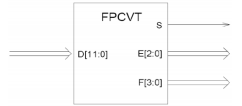
\includegraphics[width=0.8\textwidth]{fpcvtModulePic.png} 
\caption{fpcvt Module Basic Overview}
\end{center}
\end{figure}

As illustrated by the diagram above, the floating point converter module, called \textit{fpcvt} takes as input a 12 bit signal \textit{D} and outputs 3 separate signals, each a different component of the 8 bit floating point number that the module generates.  The first of the inputs \textit{S} is the sign bit. This bit is set to 0 when the number is positive and is set to 1 when the number is negative.  The second output generated is \textit{E}, a 3 bit signal representing the exponent component of the floating point number.  The third and final output generated is \textit{F}, a 4 bit signal representing the significand of the floating point number.  The resulting floating point number is therefore a combination of these three outputs and takes the following 8 bit form:

\begin{figure}[H]
\begin{center}
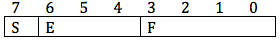
\includegraphics[width=0.8\textwidth]{floatingPointRep.png} 
\caption{fpcvt Module Basic Overview}
\end{center}
\end{figure}

The exponent and the significand work together to represent the magnitude of the number.  The significand represents the 4 most significant bits, while the exponent's purpose is to store the power to which 2 should be placed before multiplied with the significand to obtain the final magnitude of the final floating point number.  For further explanation, the resulting floating point number generated is obtained by the following formula where \textit{V} represents the final value of the generated floating point number: 

\begin{center}
\[ V  =  (-1)^S \times F \times 2^E \]
\end{center}

Some examples of this 8 bit floating point representation can be seen in the table below:

\begin{center}
\begin{tabular}{ c c c }

\textbf{Floating Point Representations}
 \textbf{Floating Point} & \textbf{Representation Formula} & \textbf{Value} \\ 
\big[0 000 0000\big] & 0 x 20 & 0\\  
\big[1 010 1010\big]  & -10 x 22 & -40 \\
\big[0 011 0111\big] & 7 x 23 & 56\\
\big[0 010 1110\big] & 14 x 22 & 56\\

\end{tabular}
\end{center}

In order to correctly implement this floating point converter, there are some special cases that must be considered.  The first of which is rounding.  This will occur quite often and must be considered.  Since the converter compresses the data from 12 bits to 8 bits, there are many numbers that cannot be represented by the final 8 bit number.  Therefore, the module must be able to handle cases where such numbers are compressed, and it does so by rounding.  In the process of conversion, the 4 most significant bits are taken and placed into the significand.  The 5th most significant bit is then taken and used to consider rounding.  If this 5th bit is 1, the significand is rounded up.  If the 5th bit is a 0, the remaining bits will be truncated, thus rounding the resultant number down.  Some examples of how the module implements rounding are included in the table below:

\begin{center}
\begin{tabular}{ c c c }

\textbf{Rounding Examples}
 \textbf{Linear Encoding} & \textbf{Floating Point Encoding} & \textbf{Rounding } \\ 
000000101100 & \big[0 010 1011\big] & Down \\
000000101101 & \big[0 010 1011\big] & Down \\ 
000000101110 & \big[0 010 1100\big] & Up \\
000000101111 & \big[0 010 1100\big] & Up \\

\end{tabular}
\end{center}

Another, but a more specific, outlying case that must be dealt with is when the significand is rounded up, but the significand consists of 4 1's. When this occurs, the exponent is incremented by 1 and the significand is first right shifted by 1 and then incremented by 1.  This successfully completes the rounding.  There is one even more specific case of rounding occurring when the exponent is incremented due to rounding, but it already contains all 1's. The converter module in this situation does not increment or shift either the exponent or the significand, because doing so would result in a garbage number.  This last example occurs when the input to the converter is too large of a number to be represented in 8 bit floating point form. Therefore, it logically follows that the final floating point number generated should have a magnitude with all 1's as this is the greatest possible magnitude that it is able to hold.

 
%----------------------------------------------------------------------------------------
%	SECTION 2
%----------------------------------------------------------------------------------------

\section*{Exercise 2 - Translate the Program}

\begin{center}
\begin{tabular}{ c c}

 \textbf{Binary} & \textbf{Sequencer Instruction} \\ 
 0000 0100 & PUSH R0 0x4 \\  
 0000 0000 & PUSH R0 0x0 \\
0001 0011 & PUSH R1 0x3 \\
1000 0110 & MULT R0 R1 R2 \\
0110 0011 & ADD R2 R0 R3 \\
1100 0000 & SEND R0 \\
1101 0000 & SEND R1 \\
1110 0000 & SEND R2 \\
1111 0000 & SEND R3 \\
 
\end{tabular}
\end{center}



%----------------------------------------------------------------------------------------
%	SECTION 3
%----------------------------------------------------------------------------------------

%----------------------------------------------------------------------------------------
%	BIBLIOGRAPHY
%----------------------------------------------------------------------------------------

%\bibliographystyle{apalike}

%\bibliography{sample}

%----------------------------------------------------------------------------------------


\end{document}